\documentclass[12pt, a4paper]{article}
\usepackage{../../../myconfig} % Gọi file cấu hình từ ngoài gốc vào

% ==========================================
% BẮT ĐẦU NỘI DUNG TÀI LIỆU
% ==========================================
\begin{document}

% Truyền 3 tham số: {Nhãn cam} {Chữ to chính giữa} {Chữ ở góc phải Header}
\titlebox{Chủ đề: Hàm số}{Tính đơn điệu của hàm số}{Hàm số: Tính đơn điệu}

\drawdashlines{29}
\newpage
\questionLinesManual{16}{1}{Cho hàm số \( y = 2x+1 \)
}

\questionLinesManual{16}{2}{Cho hàm số \( y = 2x^2-6x+1 \)
}

\questionLinesManual{16}{3}{Cho hàm số \( y = (x-1)(x-2)(x+3) \)
}

\questionLinesManual{16}{4}{Cho hàm số \( y = x^5(x-1)(x+1)^3(x-3) \)
}

\questionLinesManual{25}{5}{Cho hàm số \( y = x^2(x-2)(x-4)^4(x-3) \)

}

\newpage
\drawdashlines{35}
\newpage
\drawdashlines{35}
\newpage

\begin{center}
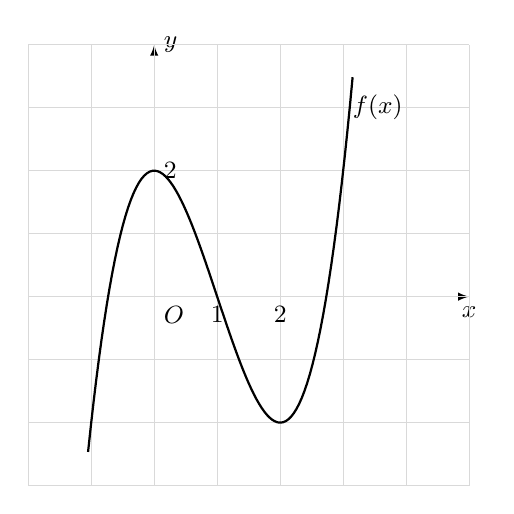
\begin{tikzpicture}[>=latex, scale=0.8]
    % Hệ trục tọa độ
    \draw[->] (-2,0) -- (5,0) node[below] {\small $x$};
    \draw[->] (0,-3) -- (0,4) node[right] {\small $y$};
    \node[below right] at (0,0) {\small $O$};
    \foreach \x in {-1,1,2,3} {
         \draw (\x,0.05) -- (\x,-0.05) ;
    }
    \foreach \y in {-2,-1,1,2,3} {
          \draw (0.05,\y) -- (-0.05,\y)   ;
    }
    \draw[color=gray!30, thin, step=1] (-2,-3) grid (5,4);
    % Đồ thị hàm bậc 3: y = -x^3 + 3x^2 + 2
    \draw[thick, samples=100, domain=-1.05:3.15] 
        plot (\x, {\x*\x*\x - 3*\x*\x + 2});
    \node[right] at (3,3) {\small $f(x)$};
    \node [below] at (1,0) {\small $1$};
   \node [below] at (2,0) {\small $2$};
   \node [right] at (0,2) {\small $2$};
\end{tikzpicture}

\end{center}
\drawdashlines{25}
\newpage

\questionLinesManual{8}{6}{Cho hàm số \( y = f(x) \) có đồ thị như hình vẽ bên. Hàm số đã cho đồng biến trên khoảng nào dưới đây?
\begin{center}
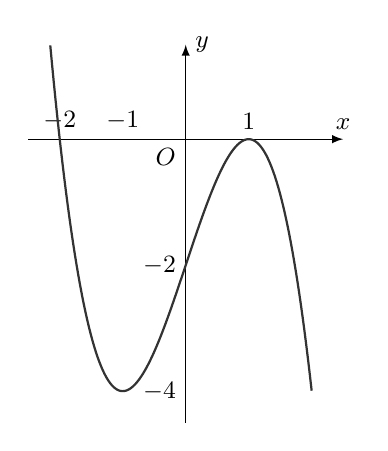
\begin{tikzpicture}[>=latex, scale=0.8]
    % Vẽ hệ trục tọa độ Ox, Oy
    \draw[->] (-2.5,0) -- (2.5,0) node[above] {\small $x$};
    \draw[->] (0,-4.5) -- (0,1.5) node[right] {\small $y$};
    \node[below left] at (0,0) {\small $O$};
    
    % Điền nhãn tọa độ trên trục chuẩn theo hình
    \node[above ] at (-2,0) {\small $-2$};
    \node[above ] at (-1,0) {\small $-1$};
    \node[above ] at (1,0) {\small $1$};
    \node[left] at (0,-2) {\small $-2$};
    \node[left] at (0,-4) {\small $-4$};
    
    % Vẽ đồ thị bằng hàm số chuẩn y = -x^3 + 3x - 2
    \draw[thick, color=black!80, samples=150, domain=-2.15:2] 
        plot (\x, {-\x*\x*\x + 3*\x - 2}); 
        
    
\end{tikzpicture}
\end{center}}


\questionLinesManual{8}{7}{Cho hàm số \( y = f(x) \) có đồ thị như hình vẽ bên. Hàm số đã cho nghịch biến trên khoảng nào dưới đây?
\begin{center}
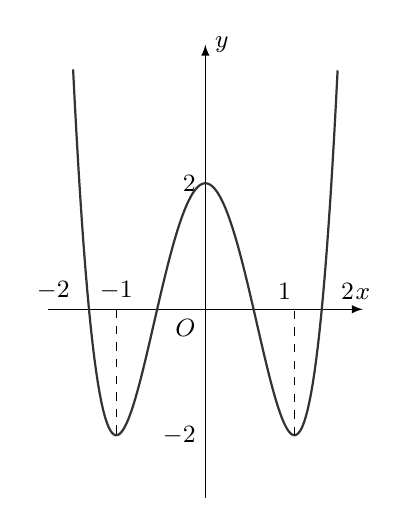
\begin{tikzpicture}[>=latex, scale=0.8]
    % Vẽ hệ trục tọa độ Ox, Oy
    \draw[->] (-2.5,0) -- (2.5,0) node[above] {\small $x$};
    \draw[->] (0,-3.0) -- (0,4.2) node[right] {\small $y$};
    \node[below left] at (0,0) {\small $O$};
    
    % Điền nhãn tọa độ chuẩn đi qua các điểm cắt Ox và Oy
    \node[above left] at (-2,0) {\small $-2$};
    \node[above left] at (-1,0) {\small $-1$};
    \node[above right] at (1,0) {\small $1$};
    \node[above right] at (2,0) {\small $2$};
    \node[left] at (0,2) {\small $2$};
    \node[left] at (0,-2) {\small $-2$};
    
    % Vẽ đồ thị dạng chữ W chuẩn bằng hàm y = x^4 - 4x^2 + 2
    \draw[thick, color=black!80, samples=150, domain=-2.1:2.1] 
        plot (\x, {\x*\x*\x*\x - 4*\x*\x + 2}); 
        
    % Đường nét đứt gióng từ cực tiểu (x = +-sqrt(2) = +-1.41) xuống y = -2 chuẩn chỉnh 100%
    \draw[dashed, line width=0.5pt] (-1.414, 0) -- (-1.414, -2) (1.414, -2) -- (1.414, 0);
\end{tikzpicture}
\end{center}}

\questionLinesManual{5}{8}{Cho hàm số \( y = f(x) \) đồ thị hàm số như hình vẽ. Hàm số đồng biến trên khoảng nào?
\begin{center}
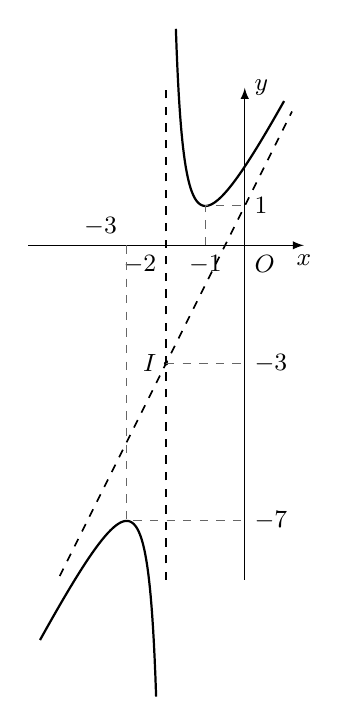
\begin{tikzpicture}[>=latex, scale=0.5]
    % Vẽ hệ trục tọa độ Ox, Oy màu đen
    \draw[->, black] (-5.5,0) -- (1.5,0) node[below] {\small $x$};
    \draw[->, black] (0,-8.5) -- (0,4.0) node[right] {\small $y$};
    \node[below right] at (0,0) {\small $O$};
    
    % Điền các nhãn tọa độ trên trục hoành và trục tung
    \node[above left] at (-3,0) {\small $-3$};
    \node[below left] at (-2,0) {\small $-2$};
    \node[below] at (-1,0) {\small $-1$};
    \node[right] at (0,1) {\small $1$};
    \node[right] at (0,-3) {\small $-3$};
    \node[right] at (0,-7) {\small $-7$};
    
    % Vẽ tiệm cận đứng (x = -2) và tiệm cận xiên (y = 2x + 1) bằng nét đứt màu đen
    \draw[dashed, black, line width=0.6pt] (-2,-8.5) -- (-2,4.0);
    \draw[dashed, black, line width=0.6pt, domain=-4.7:1.2] plot (\x, {2*\x + 1});
    \fill[black] (-2,-3) circle (1.5pt) node[left] {\small $I$}; % Tâm đối xứng I màu đen
    
    % VẼ ĐỒ THỊ MÀU ĐEN CHUẨN XÁC THEO HÀM SỐ: y = 2x + 1 + 2/(x + 2)
    % Nhánh trái (x < -2)
    \draw[thick, color=black, samples=150, domain=-5.2:-2.25] 
        plot (\x, {2*\x + 1 + 2/(\x + 2)});
        
    % Nhánh phải (x > -2)
    \draw[thick, color=black, samples=150, domain=-1.75:1.0] 
        plot (\x, {2*\x + 1 + 2/(\x + 2)});
        
    % Các đường nét đứt gióng tọa độ cực trị màu đen mảnh (light/thin)
    \draw[dashed, black!60, line width=0.4pt] (-1,0) -- (-1,1) -- (0,1);     % Cực tiểu (-1; 1)
    \draw[dashed, black!60, line width=0.4pt] (-3,0) -- (-3,-7) -- (0,-7);   % Cực đại (-3; -7)
    \draw[dashed, black!60, line width=0.4pt] (-2,-3) -- (0,-3);             % Cao độ của tâm I
\end{tikzpicture}
\end{center}}

\questionLinesManual{5}{9}{Cho hàm số \( y = f(x) \) đồ thị hàm số như hình vẽ. Hàm số đồng biến trên khoảng nào?
\begin{center}
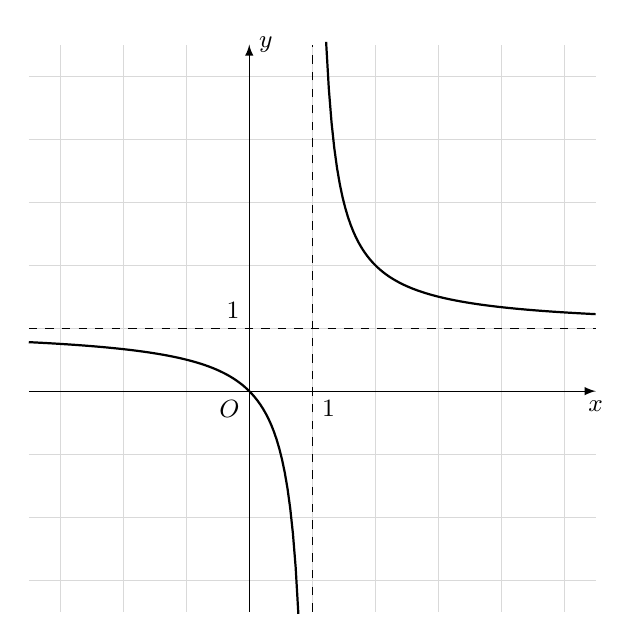
\begin{tikzpicture}[>=latex, scale=0.8]
    % 1. Vẽ lưới
    \draw[color=gray!30, thin, step=1] (-3.5,-3.5) grid (5.5,5.5);
    
    % 2. Vẽ hệ trục tọa độ
    \draw[->] (-3.5,0) -- (5.5,0) node[below] {\small $x$};
    \draw[->] (0,-3.5) -- (0,5.5) node[right] {\small $y$};
    \node[below left] at (0,0) {\small $O$};
    
    % 4. Vẽ đồ thị hàm số y = x/(x-1)
    \draw[thick, samples=100, domain=-3.5:0.78] 
        plot (\x, {\x/(\x - 1)});
    \draw[thick, samples=100, domain=1.22:5.5] 
        plot (\x, {\x/(\x - 1)});
    
    % 5. Đường tiệm cận
    \draw[dashed] (1,-3.5) -- (1,5.5);
    \draw[dashed] (-3.5,1) -- (5.5,1);
    \node[below right] at ( 1,0) {\small $1$};
    \node [ above left] at (0,1) {\small $1$};
\end{tikzpicture}
\end{center}}

\newpage
\drawdashlines{35}
\newpage

\questionLinesManual{17}{10}{Cho hàm số \( y = x^3 - 3x^2 \). Hàm số nghịch biến trên khoảng nào?
}

\questionLinesManual{17}{11}{Hỏi hàm số \( y = 2x^4 + 1 \) đồng biến trên khoảng nào?
}


\questionLinesManual{16}{12}{Cho hàm số \( y = \dfrac{x-2}{x+1} \). Hàm số đồng biến trên khoảng nào?
}


\questionLinesManual{16}{13}{Cho hàm số \( y = \dfrac{2x+3}{x-2} \). Hàm số nghịch biến trên khoảng nào?
}


\questionLinesManual{16}{14}{Cho hàm số \( y = \dfrac{x^2+2x+2}{x+1} \). Hàm số nghịch biến trên khoảng nào?
}

\questionLinesManual{16}{15}{Cho hàm số \( y = \dfrac{x^2-x+1}{x-1} \). Hàm số nghịch biến trên khoảng nào?
}

\questionLinesManual{17}{16}{Cho hàm số \( y = \sqrt{2x^2 + 1} \). xét tính đơn điệu của hàm số?}

\questionLinesManual{17}{17}{Cho hàm \( y = \sqrt{x^2 - 6x + 5} \). xét tính đơn điệu của hàm số?}

\questionLinesManual{4}{18}{Cho hàm số \( y = f(x) \) có bảng biến thiên như sau:
\begin{center}

\begin{tikzpicture}
\tkzTabInit[color, lgt=1.25, espcl=3]
{$x$ / 0.8, $f'(x)$ / 0.8, $f(x)$ / 2}
{$-\infty$, $-1$, $0$, $1$, $+\infty$}
\tkzTabLine{ , +, 0, -, 0, + }
\tkzTabVar{-/$-\infty$, +/$2$, -/$1$, +/$2$, -/$-\infty$}
\end{tikzpicture}
\end{center}
Hàm số đã cho đồng biến trên khoảng nào?}

\questionLinesManual{4}{19}{Cho hàm số \( y = f(x) \) có bảng biến thiên như hình dưới đây. Xét tính đơn diệu của hàm số?
\begin{center}

\begin{tikzpicture}
\tkzTabInit[color, lgt=1.25, espcl=3]
{$x$ / 0.8, $y'$ / 0.8, $y$ / 2}
{$-\infty$, $-\dfrac{1}{2}$, $3$, $+\infty$}
\tkzTabLine{ , +, d, +, 0, - , }
\tkzTabVar{-/ $-\infty$, +D-/ $+\infty$ / $-\infty$, +/ $4$, -/ $-\infty$}
\end{tikzpicture}
\end{center}}


\questionLinesManual{3}{20}{Cho hàm số \( y = f(x) \) có bảng xét dấu đạo hàm như sau:
\begin{center}

\begin{tikzpicture}
\tkzTabInit[color, lgt=1.25, espcl=2.5]
{$x$ / 0.8, $y'$ / 0.8}
{$-\infty$, $-2$, $0$, $2$, $+\infty$}
\tkzTabLine{ , +, 0, -, d, -,0,+}
\end{tikzpicture}
\end{center}
Xét tính đơn điệu của hàm số?}

\questionLinesManual{3}{21}{Cho hàm số \( y = f(x) \) có bảng xét dấu của đạo hàm như hình vẽ.
Hàm số đã cho nghịch biến trên khoảng nào?
\begin{center}

\begin{tikzpicture}
\tkzTabInit[color, lgt=1.25, espcl=2.5]
{$x$ / 0.8, $y'$ / 0.8}
{$-\infty$, $-1$, $1$, $+\infty$}
\tkzTabLine{ , -, d, -, 0 ,+}
\end{tikzpicture}
\end{center}}

\newpage
\drawdashlines{35}
\newpage

\questionLinesManual{16}{22}{Cho hàm số \( y = f(x) \) liên tục trên \( \mathbb{R} \) và có đạo hàm  
\( f'(x) = (1 - x)^2 (x + 1)^3 (3 - x). \)  
Hàm số \( y = f(x) \) đồng biến trên khoảng nào dưới đây?}


\questionLinesManual{15}{23}{Cho hàm số \( y = f(x) \) có đạo hàm \( f'(x) = x(x - 2)^3 \), với mọi \( x \in \mathbb{R} \). Hàm số đã cho nghịch biến trên khoảng nào?}


\questionLinesManual{30}{24}{Cho hàm số \( f(x) \) liên tục trên \( \mathbb{R} \) có đạo hàm  
\( f'(x) = (x+2)(x-1), \forall x \in \mathbb{R}. \) 
Hàm số đã cho nghịch biến trên khoảng nào?}

\begin{center}
    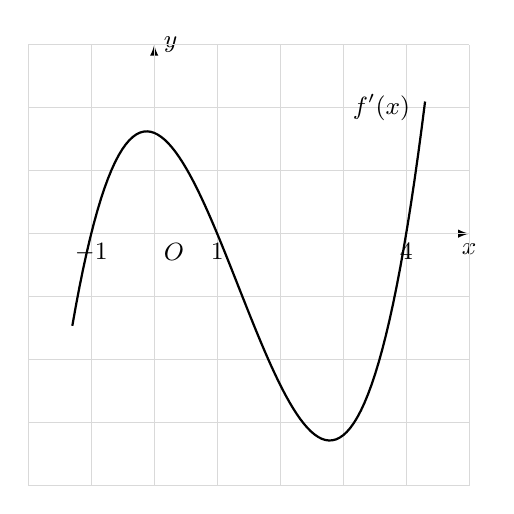
\begin{tikzpicture}[>=latex, scale=0.8]
    % Hệ trục tọa độ
    \draw[->] (-2,0) -- (5,0) node[below] {\small $x$};
    \draw[->] (0,-4) -- (0,3) node[right] {\small $y$};
    \node[below right] at (0,0) {\small $O$};
    \foreach \x in {-1,1,2,3} {
         \draw (\x,0.05) -- (\x,-0.05) ;
    }
    \foreach \y in {-2,-1,1,2,3} {
          \draw (0.05,\y) -- (-0.05,\y)   ;
    }
    \draw[color=gray!30, thin, step=1] (-2,-4) grid (5,3);
    % Đồ thị hàm bậc 3: y = -x^3 + 3x^2 + 2
    \draw[thick, samples=100, domain=-1.3:4.3] 
        plot (\x, {0.4*(\x+1)*(\x-1)*(\x-4)});
    \node[right] at (3,2) {\small $f'(x)$};
   \node [below] at (1,0) {\small $1$};
   \node [below] at (4,0) {\small $4$};
   \node [below] at (-1,0) {\small $-1$};
\end{tikzpicture}
\end{center}
\drawdashlines{25}
\newpage

\questionLinesManual{8}{25}{Cho hàm số \( y = f(x) \) xác định, có đạo hàm trên \( \mathbb{R} \) và \( f'(x) \) có đồ thị như hình vẽ bên dưới
\begin{center}
\begin{tikzpicture}[>=latex, scale=1]
    % Hệ trục tọa độ
    \draw[->] (-4.5,0) -- (4.5,0) node[below] {\small $x$};
    \draw[->] (0,-3.5) -- (0,1.5) node[right] {\small $y$};
    \node[above left] at (0,0) {\small $O$};
    
    % Vẽ đồ thị f'(x) là parabol hướng lên có nghiệm tại x = -3 và x = 1
    \draw[thick, color=black!80, samples=150, domain=-3.2:0.7] 
       plot (\x, {-0.5*(\x*\x*\x*\x + 5*\x*\x*\x + 6*\x*\x)}); 
        
    % Ký hiệu tên hàm số f'(x) ở góc phải bên dưới
    \node[right] at (0.5,-3.0) {\small $f'(x)$};
    
    % Đánh dấu các điểm trên trục Ox
    \node[below] at (-3,0) {\small $-3$};
    \node[below] at (1,0) {\small $1$};
    \node[above right] at (-2,0) {\small $-2$};
\end{tikzpicture}
\end{center}
Xét tính đơn điệu của hàm số trên?}


\questionLinesManual{7}{26}{Cho hàm số \( y = f(x) \) xác định, có đạo hàm trên \( \mathbb{R} \) và \( f'(x) \) có đồ thị như hình vẽ bên dưới
\begin{center}
\begin{tikzpicture}[>=latex, scale=0.8]
    % Hệ trục tọa độ
    \draw[->] (-4.5,0) -- (4.5,0) node[below] {\small $x$};
    \draw[->] (0,-5) -- (0,2) node[right] {\small $y$};
    \node[above left] at (0,0) {\small $O$};
    
    % Vẽ đồ thị f'(x) là parabol hướng lên có nghiệm tại x = -3, x = -1, x = 2
    \draw[thick, color=black!80, samples=150, domain=-2.2:2.4] 
       plot (\x, {-0.5*\x*\x*\x*\x + 0.5*\x*\x*\x + 3*\x*\x - 2*\x - 4});
    
    % Đánh dấu các điểm trên trục Ox
    \node[above left] at (-2,0) {\small $-2$};
    \node[above left] at (-1,0) {\small $-1$};
    \node[left] at (0,-4) {\small $-4$};
    \node[above] at (2,0) {\small $2$};
\end{tikzpicture}
\end{center}
Xét tính đơn điệu của hàm số?}

\end{document}